\documentclass[fullscreen=true, bookmarks=false]{beamer}
\usepackage[utf8]{inputenc}
\usepackage[russian]{babel}
%\usepackage[14pt]{extsizes}
\usepackage{adjustbox}
\usepackage{graphicx}
\usepackage{amsmath,amsfonts,amssymb,amsthm,mathtools} 
\usepackage{ulem}
\usepackage[backend=biber]{biblatex}
\usepackage[top=2cm,bottom=2cm,left=2cm,right=1cm,nohead,nofoot]{geometry}
\usepackage[onehalfspacing]{setspace}
\usepackage{ifthenx}
\usepackage{ifthen}
\usepackage{tikz}
\usetikzlibrary{arrows,positioning,shadows,datavisualization}
\usepackage[
bookmarks=true, colorlinks=true, unicode=true,
urlcolor=black,linkcolor=black, anchorcolor=black,
citecolor=black, menucolor=black, filecolor=black,
]{hyperref}
\usepackage{microtype}
\usepackage{enumerate}
\usepackage{multirow}
\usepackage{paralist,array}
\usepackage{blindtext}
\usepackage{newfloat}
\usepackage{verbatim}
\usepackage{ragged2e}

\setlength{\parskip}{0ex} 

\usetheme{CambridgeUS}

\title{Сервис для разметки данных}
\author{Рязанов М.С.\\ИУ7--62Б}

\begin{document}

\begin{frame}
	Курсовой проект по дисциплине <<Базы данных>>:
    \begin{center}
    \Huge
    Сервис для разметки данных
    \end{center}

    \large
    Руководитель курсового проекта: Ковтушенко Александр Петрович

    Студент: Рязанов Максим Сергеевич

    Группа: ИУ7--62Б

\end{frame}

\section*{План презентации}

\begin{frame}
\frametitle{Содержание}
\tableofcontents
\end{frame}

\section{Введение}
\subsection{Цели и задачи}

\begin{frame}
	\begin{center}
		\large
		Цели и задачи
	\end{center}
	\begin{enumerate}
		\item Выделить основные сущности предметной области;
    	\item На основе выделенных сущностей разработать схему базы данных;
    	\item Разработать иерархию классов бизнес-логики и доступа к данным;
    	\item Разработать интерфейс веб-приложения;
    	\item Реализовать веб-приложение;
    	\item Обеспечить тестирование реализованного приложения;
	\end{enumerate}
\end{frame}


\section{Аналитический раздел}

\subsection{Сущности}
Были выделены следующие сущности

\begin{itemize}

\item Проект

Сущность, определяющая набор данных одного типа и одного типа разметки, относящихся к одной тематике.

\item Пользователь

Сущность, которая содержит информацию о пользователе: администраторе или обычном.
Может иметь привелегии относящиеся к различным проектам.

\item Привелегия (право)

Сущность, которая контролирует возможности пользователей 
размечать данные определенного проекта.

\item Элемент выборки

Сущность, содержащая информацию о конкретном элементе данных, принадлежащих проекту.

\item Метка

Ответ пользователя данный им в процессе разметки для конкретного элемента выборки.

\item Схема проекта
Сущность, содержащая информацию о множестве допустимых значений элементов выборки и меток.

\item Сессия

Сущность, содержащая информацию о подключении пользователя.

\end{itemize}

\subsection{Роли}
Для пользователей приложения выделены следующие роли:

\begin{itemize}
\item Администратор

Имеют возможность создавать проекты, загружать выборку и выгружать метки для созданных ими проектов, предоставлять и лишать
других пользователей привелегий для разметки принадлежащих им проектов, осуществлять разметку проектов к которым имеют привелегии.

\item Обычный пользователь 
Имеют возможность осуществлять разметку данных проектов, в соответствии с привелегиями, предоставленными администраторами. 

\end{itemize}

\begin{figure}
    \caption{Use-Case диаграма}
    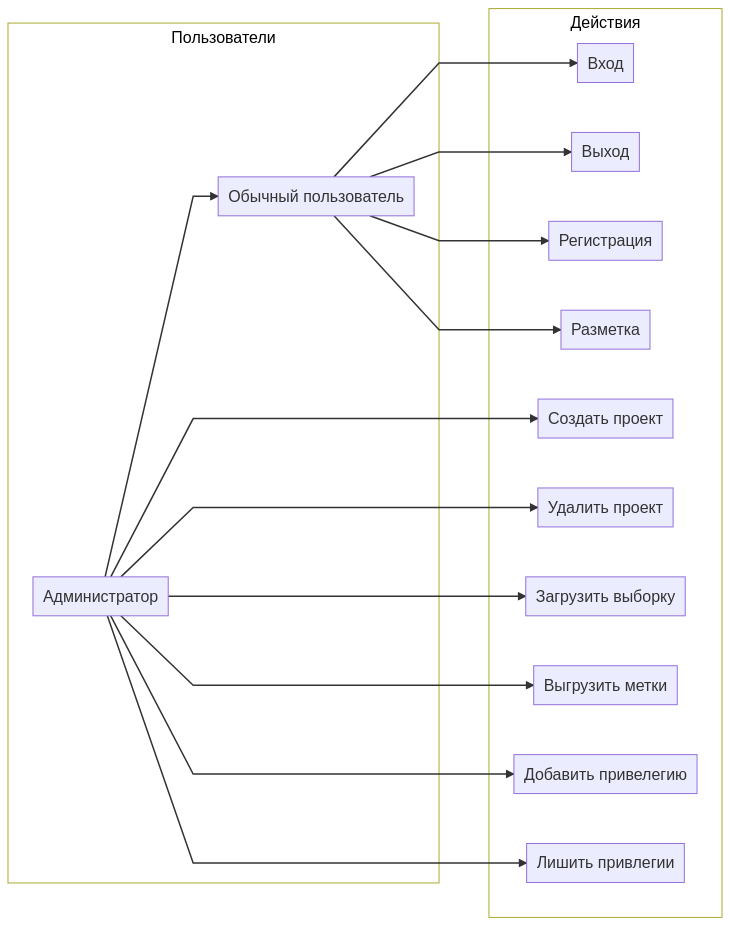
\includegraphics[width=0.9\textwidth]{./use-case.png}
\end{figure}


\section{Конструкторский раздел}

\subsection{Модели базы данных}

\begin{frame}

\begin{itemize}
    \item Users --- таблица с данными о пользователях.
    \item Projects --- таблица с основными данными о проектах.
    \item ProjectSchemas --- таблица с данными о схемах проектов.
    \item ProjectGrants --- таблица с данными о возможности пользователей размечать данные проектов.
    \item Tasks --- таблица с данными о элементах выборки
    \item LabeledTasks --- таблица с данными о метках
    \item Sessions --- таблица с данными о сессиях пользователей
\end{itemize}


\end{frame}

\subsection{Схема базы данных}

\begin{frame}
    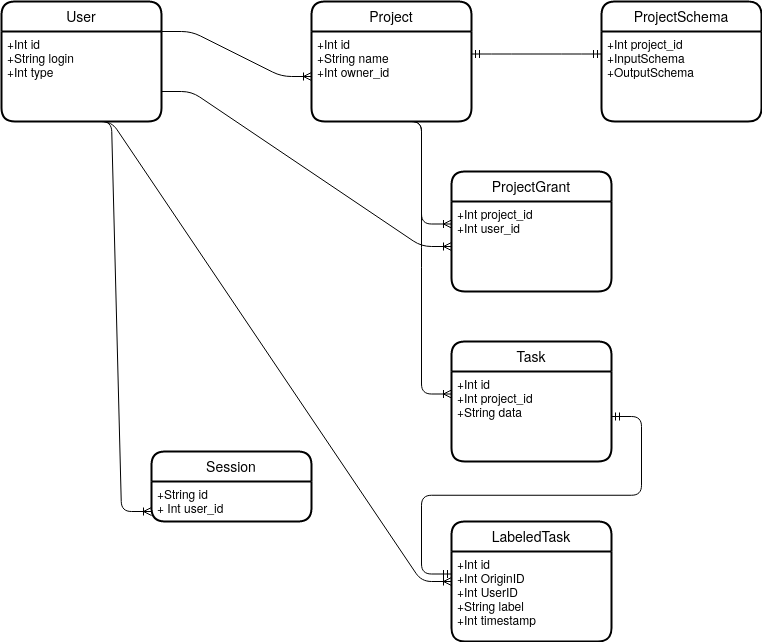
\includegraphics[width=0.8\textwidth]{./dbschema.png}
\end{frame}


\subsection{Классы компоненты доступа к данным}
\begin{frame}
    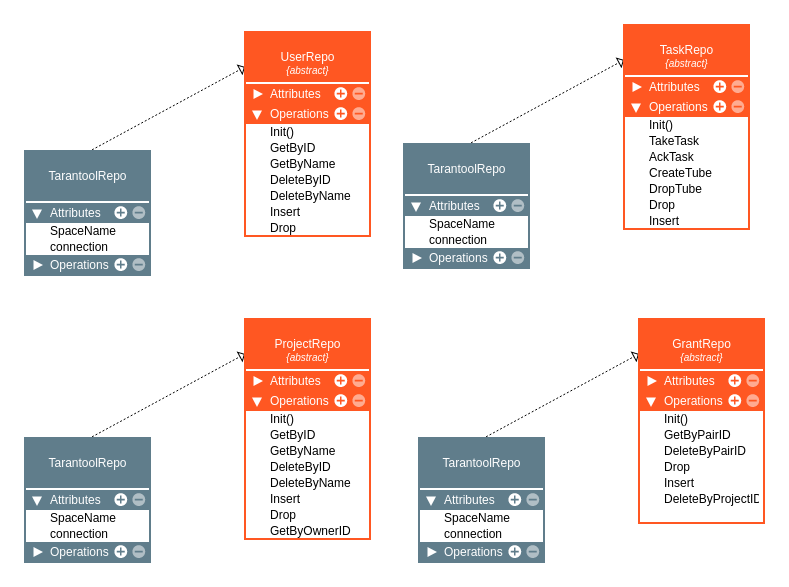
\includegraphics[width=0.9\textwidth]{./dataaccess.png}
\end{frame}

\subsection{Классы компоненты бизнес-логики}

\begin{frame}
    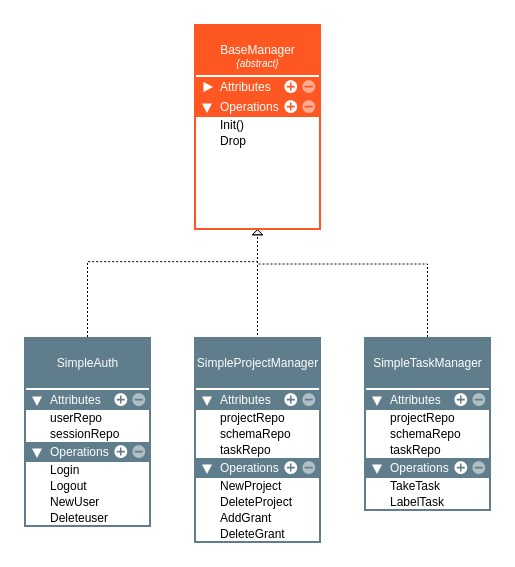
\includegraphics[width=0.8\textwidth]{./business.png}
\end{frame}

\subsection{Классы схем данных}

\begin{frame}
    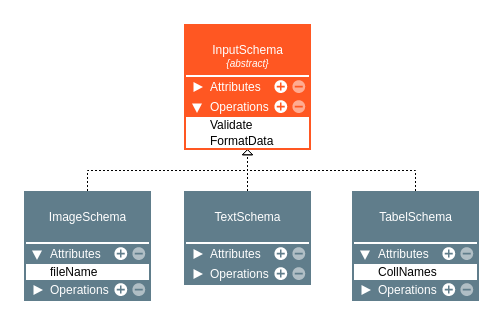
\includegraphics[width=0.9\textwidth]{./inputschema.png}
\end{frame}

%\subsection{Диаграмма классов представлений}

%\begin{frame}
%    \includegraphics[width=1\textwidth]{./views2.png}
%\end{frame}


\section{Технологический раздел}

\subsection{Серверная часть}

Ниже приведены технологии, которые были использованы в серверной части приложения

\begin{itemize}
    \item Go 1.15\cite{godoc} --- язык программирования. 
    Он имеет достаточно много удобных библиотек для веб-разработки и
    обширное сообщество, что уменьшает вероятность возникновения 
    трудноразрешимых проблем, ускоряет разработку и позволяет 
    сконцентрироваться на архитектуре проекта.

    \item Tarantool 2.2.4\cite{tarantooldoc} --- Резидентная СУБД и сервер приложений.
    Приемуществами является скорость работы, 
    огромное количество возможностей,
    хорошая документация и открытый исходный код.
    Недостатков замечено не было.

    \item Go-tarantool\cite{go-tarantool} --- Библиотека для подключения к Tarantool из Go.
    
    \item TarantoolQueue\cite{tarantooldoc} --- Модуль консистентных 
    очередей для Tarantool.

    Использовался для обеспечения консистентной обработки запросов на разметку, предотвращения 
    повторной разметки одного
    элемента выборки.
    
    \item TarantoolDDL\cite{tarantooldoc} --- Модуль декларативного описания таблиц в Tarantool. 
\end{itemize}

\subsection{Клиентская часть}

Инструменты, использованные для браузерной части приложения

\begin{itemize}
    \item HTML5 --- язык разметки веб-страниц.
    
    \item GoTemplates --- язык шаблонов для HTML страниц. Использовался для создания динамических веб-страниц.\cite{gotemplate}

    \item CSS --- язык стилей, предоставляет широкие возможности по 
            манипуляции внешним видом веб-страницы.

    \item JavaScript --- язык программирования, который широко 
        используется для создания интерактивных и динамических 
        веб-страниц.  

    \item Bootstrap\cite{bootstrap4docs} --- Css-фреймфорк, 
        который предоставляет большое количество готовых
        CSS классов, что значительно ускоряет создание
        современного интерфейса.
\end{itemize}

\subsection{Структура проекта}

\begin{itemize}
    \item Models --- модуль, содержащий реализацию сущностей приложения на языке Go.
    \item Auth ---   модуль, авторизации
    \item Repos --- модуль, содержащий логику доступа к данным
        \item Grant --- модуль доступа к данным привелегий
        \item LabeledTask --- модуль доступа к размеченным данным
        \item Project --- модуль доступа к данным проекта
        \item Schema --- модуль доступа к схемам проектов
        \item Session --- модуль доступа к сессиям пользователей
        \item Task --- модуль доступа к размечаемым данным
        \item User --- модуль доступа к данным пользователей
    \item Universe --- модуль - глобальный репозиторий, обеспечивающий централизованную работу с подключениями к базе данных
    \item Tarantool --- модуль обеспечивающий загрузку СУБД Tarantool, создание таблиц, загрузку хранимых процедур на Lua.
\end{itemize}




\section{Эксперементальный раздел}

\subsection{Демонстрация GUI}

\begin{frame}
    \frametitle{Cоздание проекта}
    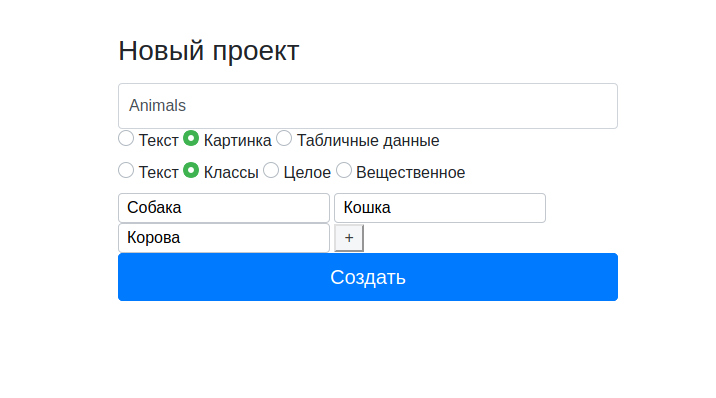
\includegraphics[width=0.9\textwidth]{./create_project.png}
\end{frame}


\begin{frame}
    \frametitle{Разметка изображений}
    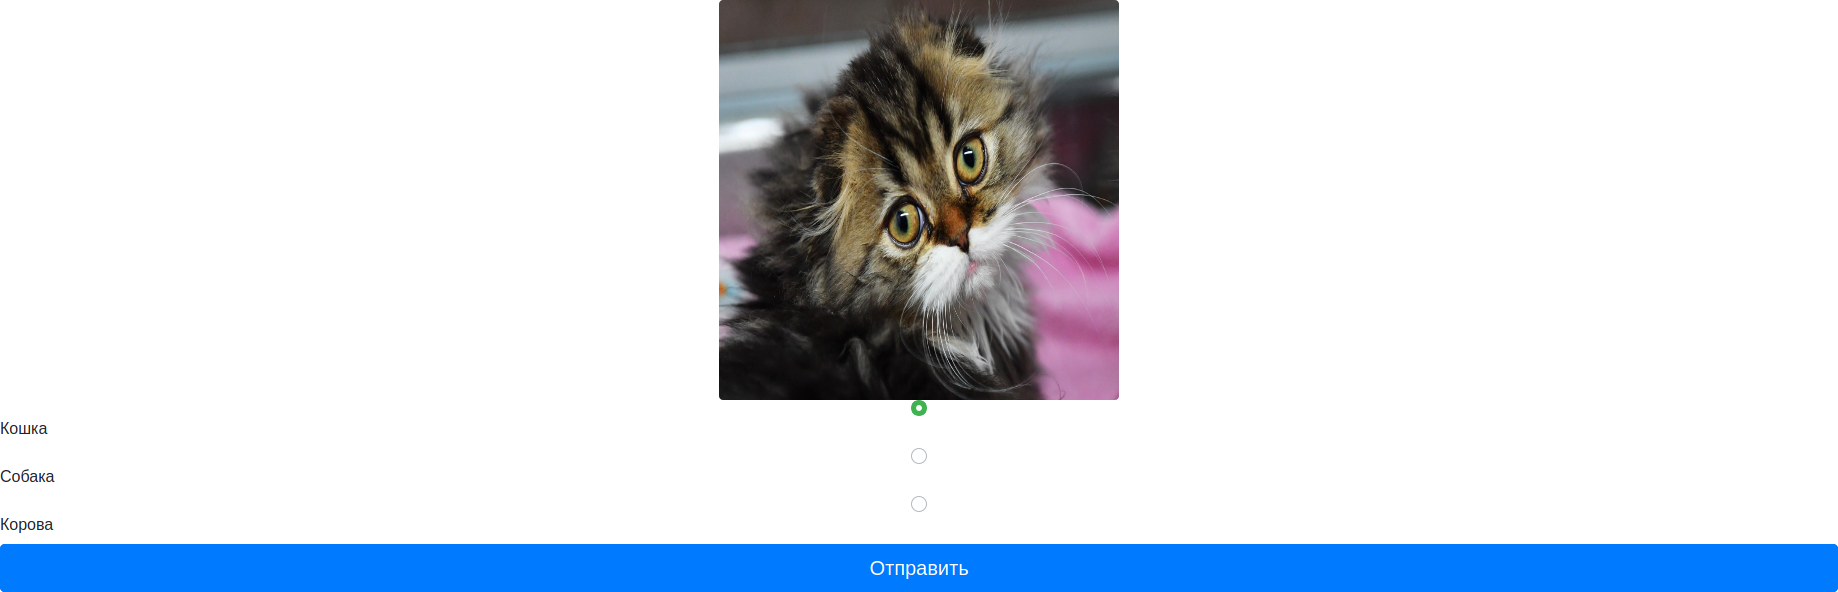
\includegraphics[width=0.9\textwidth]{./animalslabel.png}
\end{frame}

\begin{frame}
    \frametitle{Разметка табличных данных}
    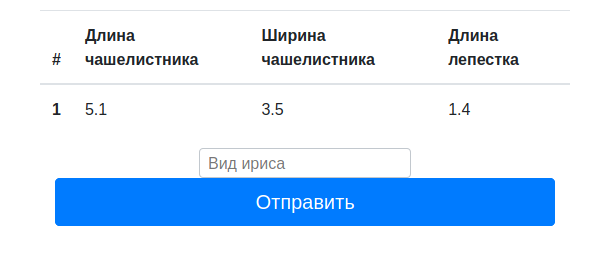
\includegraphics[width=0.9\textwidth]{./tablelabel.png}
\end{frame}


\section*{Перспективы развития}
\subsection*{Перспективы развития}
\begin{frame}
    Могут быть предложены следующие перспективы развития проекта
    \begin{itemize}
        \item Расширение видов входных данных: видео, ссылки на сторонние ресурсы
        \item Расширение возможных видов разметки: прямоугольная область для изображений, временной промежуток(для видео)
        \item Добавление возможности устанавливать денежное вознаграждение за разметку проекта
    \end{itemize}
\end{frame}
\end{document}
